\label{soluzione_problematiche}
\subsection{Entit\`{a} Circuito}
\label{entita_circuito}
Nella soluzione proposta il circuito è un'unità composta da più entità passive
ad accesso mutuamente esclusivo. Più precisamente:
\begin{itemize}
\item \textbf{Path}: rappresenta la traiettoria percorsa da un concorrente. Un
insieme di \textbf{Path} costituisce un tratto e il loro
numero all'interno del tratto identifica le possibili vie che si possono intraprendere per attraversarlo. 
Ogni path ha una molteplicità limitata da\\
\emph{lunghezza / 4.5}\\
dove 4.5 è lo spazio longitudinale richiesto da un'auto di formula 1 per non entrare in collisione con altre auto. Per ``\emph{molteplicità}
si intende il numero di auto che possono restare in fila all'interno di una traiettoria.
Il \textbf{Path} è caratterizzato da:
\begin{itemize}
\item lunghezza
\item angolo
\item tenuta
\item istanti di liberazione, ovvero gli istanti di tempo 
in cui le ultime \emph{N} auto che sono entrate nella traiettoria (con \emph{N} pari alla molteplicità del \textbf{Path}) sono previste uscirne;
\item istante di liberazione, ovvero l'istante in cui il tratto è previsto essere libero da tutte le auto;
\item massima velocità raggiungibile, determinata dal concorrente che è entrato più recentemente nel \textbf{Path}.
Questo valore viene usato per limitare la velocità di un concorrente nel caso esso entri quando altre auto lo stanno
attraversando.
\end{itemize}
I \textbf{Path} di uno stesso tratto possono essere uguali o differire per
caratteristiche, rimanendo comunque entro i limiti globali del tratto
(non si potrà ad esempio avere un \textbf{Path} lungo 11 km in un tratto lungo 42 m).
\item \textbf{Checkpoint}: è una risorsa passiva ad accesso mutuamente
esclusivo. Rappresenta la coda di accesso ad un tratto. Ogni posizione
della coda è stata arricchita con delle informazioni che aiutano a gestire
l'accesso al tratto:
\begin{itemize}
\item \textbf{istante di arrivo}: l'istante di tempo più ottimista in cui l'auto
è prevista arrivare oppure l'istante in cui l'auto realmente
arriva al tratto (in base al valore della flag ``arrivato'', descritta in
seguito);
\item \textbf{id concorrente}: l'id del concorrente presente nella posizione
della coda;
\item \textbf{flag ``arrivato''}: se valorizzata con \emph{true}, significa che
il concorrente sta effettivamente attendendo di accedere al tratto
e che il valore temporale segnato nell'\textbf{istante di arrivo} è l'istante di
arrivo effettivo. Altrimenti significa che il concorrente non
è ancora arrivato ma arriverà ad un istante maggiore o uguale a quello segnato
nell'\textbf{istante di arrivo}.
\end{itemize}
Ogni \textbf{Checkpoint} inoltre punta ad un insieme di \textbf{Path}.
\item \textbf{Racetrack iterator}: ogni concorrente dispone di un'istanza di
questo iteratore per poter navigare il circuito e richiedere
di accedere eventualmente ai box.
\end{itemize}
La struttura è stata pensata principalmente per venire a capo del problema dei
sorpassi impossibili.\\
Come visto nella sezione \ref{tempo}, non esiste un orologio assoluto. Ogni
concorrente segna sulla
coda il tempo di arrivo in base ai tempi accumulati per l'attraversamento dei
tratti precedenti. Quindi si può dire che ogni
concorrente aggiorni un proprio orologio relativo all'andamento della sua corsa.
Inoltre ogni concorre segna
un tempo ottimistico di arrivo sui checkpoint che (salvo ritiro) attraverserà.
Tale istante sarà di sicuro maggiore dell'istante segnato
nel \textbf{Checkpoint} in cui il concorrente effettivamente è arrivato. Questo
permette ad ogni concorrente di sapere, quindi, non solo
i dettagli relativi alla sua corsa, ma anche quelli relativi agli altri
concorrenti (quando necessario). Di conseguenza, se un concorrente
è interessato ad attraversare un tratto, potrà confrontare il suo tempo di
arrivo effettivo con i tempi di arrivo effettivi e previsti
degli altri concorrenti. Nel momento in cui il suo istante di arrivo effettivo
risulti cronologicamente il più basso della coda, sarà certo
che, stando al suo istante di tempo e a quello relativo agli altri concorrenti,
il suo turno per attraversare sia arrivato (verrà dimostrato formalmente in seguito). Ovvero che, in 
termini di tempo relativi, il suo istante, essendo il più basso, indica che è
il primo arrivato al tratto in quell'istante, avendo così
il diritto di accesso.\\
Quando un concorrente deve valutare la traiettoria (\textbf{Path}) da
attraversare in un tratto, può farlo semplicemente valutando le caratteristiche
del tratto. Le prime tre elencate qualche riga più sopra garantiscono un minimo
di realismo fisico nell'interazione concorrente-ambiente statico. Le caratteristiche fisiche del tratto infatti
influiranno sui consumi e i tempi dell'auto. Il concorrente dovrà scegliere in
modo da minimizzare entrambi.\\
Gli ultimi parametri sono anche oggetto di valutazione in quanto servono all'utente per
verificare lo stato di occupazione del tratto.\\
Un concorrente può certamente decidere di attraversare il tratto utilizzando una traiettoria
su cui sia già presente un altro concorrente. Ma ne conseguirà che se il concorrente
più veloce è dietro, esso verrà limitato dalla velocità di quello davanti.\\
Altra questione importante riguarda i tempi di liberazione: come già detto, una
traiettoria può essere contemporaneamente occupata da al più N (con N limitato) macchine.
Quando un concorrente inizia a percorrere una traiettoria, dovrà salvare in una posizione
libera della lista dei tempi di liberazione il proprio istante di uscita dal tratto.
Quando un concorrente vuole iniziare a percorrere una traiettoria, di conseguenza, dovrà verificare
che il suo tempo di arrivo sia maggiore almeno di uno dei tempi di liberazione segnati
nella lista. Solo in questo caso potrà essere certo che la traiettoria può ospitare auto.
Se tutte le traiettorie di un tratto sono sovraffollate, il concorrente dovrà
uscire di pista per evitare una collisione e si dovrà quindi ritirare.\\
Questo garantisce il realismo fisico
concorrente-concorrenti descritto nella sezione \ref{analisi_realismo_fisico}.
I tempi segnati nelle code invece mettono in pratica, in parte, il concetto di
orologio relativo enunciato nella sezione \ref{tempo}.
Maggiori dettagli sull'interazione fra concorrenti e circuito e sull'algoritmo
che regola l'attraversamento del circuito da parte dei concorrenti
verranno forniti nelle sezioni seguenti.
\subsection{Entit\`{a} Concorrente}
Il concorrente è un'entità attiva, concepita
come un task che utilizza l'entità \textbf{Circuito} per iterare sulla pista. In
seguito
verranno analizzate le interazioni che questa entità hanno fra di loro e con le
entità passive che compongono il circuito.
Questa componente è composta principalmente da tre parti che sono:
\begin{itemize}
\item Car : oggetto che rappresenta l'auto con tutte le caratteristiche
\item Driver : oggetto che rappresenta il pilota
\item Competitor\_Details : oggetto che rappresenta il concorrente nel suo
insieme, ovvero auto, pilota e componenti di strategia e di monitoraggio
\end{itemize}
\subsection{Interazione concorrenti - circuito}
I concorrenti (entità attive)
utilizzano il circuito per gareggiare nella competizione.
Ogni concorrente per gareggiare deve riuscire a ottenere il tratto di pista che
vuole attraversare. La struttura di chiamate (insieme alla struttura del
circuito già descritta nel paragrafo \ref{entita_circuito}) è stata studiata per
evitare le possibili situazioni di stallo e di sorpasso impossibile oltre che mantenere
coerenza temporale nel corso della gara. 
Ogni concorrente utilizza un iteratore (\textbf{Racetrack\_Iterator}) per iterare
attraverso i tratti della pista. Grazie ad esso il concorrente può ottenere il
\textbf{Checkpoint} del circuito nell'ordine stabilito dalla configurazione.
Può inoltre ottenere informazioni relative al tratto di entrata e uscita ai box, oltre
che ottenere il \textbf{Checkpoint} relativo ai box.\\
Come visto nella sezione \ref{entita_circuito}, i checkpoint espongono delle code
per gestire l'accesso al tratto. Per attraversare un tratto di
pista il concorrente dev'essere il primo nella coda. Una volta che un concorrente si trova nella prima posizione
della coda può utilizzare la risorsa passiva in mutua esclusione che rappresenta
il pezzo di pista. Le operazioni di calcolo dei tempi e di scelta delle
traiettorie avvengono mantenendo il possesso della risorsa, con la certezza che
nessuno modifichi le condizioni che si stanno valutando. Si evita inoltre che un concorrente
possa valutare l'attraversamento del tratto quando spetterebbe (per motivi temporali) ad un
altro concorrente.\\
Successivamente verrà spiegato più formalmente quanto detto.\\
Vediamo ora l'algoritmo per l'attraversamento di un
tratto dal momento in cui il concorrente arriva 
fisicamente ad un checkpoint
fino al raggiungimento di quello successivo.\\
Per chiarezza, la spiegazione verrà scomposta in due parti che poi, integrate,
formeranno l'algoritmo completo.
\begin{description}
\item{\textbf{Scelta traiettoria (Path):}}\\
In questo passo della simulazione, il concorrente ha già ottenuto accesso esclusivo alla collezione di \textbf{Path} e potrà quindi
effettuare la valutazione senza rischio di race condition (il perché verrà spiegato successivamente). L'algoritmo procede quindi nel
seguente modo:
\begin{itemize}
\item Per ogni traiettoria (\textbf{Path}) a disposizione:
\begin{itemize}
\item Calcola il tempo di attraversamento (in assenza di auto sulla traiettoria);
\item Confronta l'istante di uscita dato con tempo di attraversamento calcolato con l'istante di liberazione
segnato sul tratto;
\item Se l'istante di liberazione è inferiore (il che significa che il tratto è già libero quando l'auto proverà ad attraversarlo),
salva l'istante di uscita associato al \textbf{Path} come \emph{istante di arrivo} + \emph{tempo di attraversamento};
\item Se l'istante di liberazione invece è superiore, verifica se ci sia spazio per entrare nella traiettoria. Per fare ciò, bisogna considerare
la lista di istanti di liberazione. Se tutti gli istanti segnati sono maggiori dell'\emph{istante di arrivo} del concorrente, significa che 
non sarà possibile usare quella traiettoria.\\
In caso contrario, il concorrente può attraversare mettendosi dietro alla/e auto già presente/i nella traiettoria. Per questo la velocità
sarà limitata da quella dell'auto davanti e l'istante di uscita associato al path 
corrisponderà all'istante di uscita della macchina entrata più di recente (ovvero
\emph{l'istante di liberazione del tratto}) + \emph{il tempo che rappresenta la distanza minima fra due auto per evitare tamponamenti} 
(costante).
\end{itemize}
\item Se almeno un \textbf{Path} è percorribile, 
\begin{itemize}
\item scegli quello ottimo (con istante di uscita minore);
\item aggiorna il tempo di liberazione del tratto con quello appena calcolato;
\item aggiorna la lista degli istanti di liberazione aggiungendo quello nuovo in una posizione il cui istante segnato sia inferiore all'istante
di arrivo del concorrente (significa che quell'istante è già passato e non è più utile ai fini della valutazione dell'affollamento
della traiettoria);
\end{itemize}
\item Altrimenti l'utente deve uscire dal circuito per evitare collisioni, dovendo così ritirarsi.
\end{itemize}
\item{\textbf{Attraversamento tratto:}}\\
\emph{Premessa}: un concorrente arrivato effettivamente su una coda ma non primo, si mette in attesa. 
Verrà risvegliato automaticamente dall'ultimo concorrente che avrà \textbf{modificato l'ordine} della coda nel
caso risultasse primo dopo l'aggiornamento.\\
\emph{Precondizione}: il concorrente ha gi\`{a} segnato il suo tempo di arrivo
effettivo sulla coda del checkpoint che vuole attraversare.
\begin{enumerate}
\item il concorrente setta la flag ``arrivato'' nella coda del checkpoint sulla
posizione a lui riservata;
\item controlla in che posizione \`{e} nella coda;
\item se non \`{e} primo, attende di essere primo;
\item quando \`{e} primo, richiede l'insieme di traiettorie (\textbf{Path}) da
cui \`{e} costituito il tratto;
\item Calcola la traiettoria (\textbf{Path}) di attraversamento ottimale secondo l'algoritmo spiegato precedentemente.
Si otterrà quindi un istante di uscita, che corrisponderà al tempo di arrivo effettivo al checkpoint successivo;
\item segna il tempo di arrivo effettivo sulla coda del checkpoint successivo, che verr\`{a}
\textbf{riordinata} in base al nuovo tempo.
\item segna il tempo di arrivo limite su tutte le altre code (aggiungendo il minimo tempo richiesto dall'auto
per andare da un checkpoint a quello successivo), da quella
successiva al checkpoint che si sta per raggiungere a quella del checkpoint
appena attraversato. Ad ogni aggiornamento del tempo limite, la coda viene
\textbf{riordinata}.
\item Se nella coda del checkpoint l'istante di arrivo limite del concorrente risulterà maggiore di qualche altro, 
verrà riordinato in una posizione inferiore, lasciando eventualmente spazio
ad altri di effettuare valutazioni su quel tratto.
\item delay per fini di simulazione;
\item ritorna al passo 1 per il checkpoint successivo;
\end{enumerate}
\end{description}
Il diagramma di sequenza \ref{arriveAndCross} in appendice esplica a livello implementativo come l'attraversamento avviene.
La strategia adottata si presta a simulare la corsa garantendo che un concorrente possa tenere in considerazione ad
ogni istante le auto presenti sulla pista e sui tratti senza comportamenti
anomali. \`{E} necessario, tuttavia, dimostrare che l'algoritmo sia corretto. Per farlo bisogna provare che i concorrenti
non collidano (logicamente) nel corso dell'esecuzione. Ovvero:
\begin{itemize}
\item L'aggiornamento delle code sia mutuamente esclusivo
\item La valutazione di un tratto sia effettuata in modo esclusivo;
\end{itemize}
Dimostriamo che quanto detto accade:
\begin{itemize}
\item \emph{quando un concorrente valuta le traiettorie, lo sta facendo in modo
esclusivo}.
Perché due concorrenti \emph{x} e \emph{y} possano iniziare a valutare le traiettorie del tratto \emph{n}
contemporaneamente, deve verificarsi una delle seguenti due condizioni:\\
\textbf{Condizione 1}:
\begin{itemize}
\item entrambi i concorrenti sono effettivamente presenti sulla coda del \textbf{Checkpoint} e in attesa di attraversare;
\item i due concorrenti \emph{x} e \emph{y}, ordinati nella coda per tempo di arrivo crescente, hanno assegnati rispettivamente i tempi
\emph{$t_x$} e \emph{$t_y$}, con $t_x$ < $t_y$; per come è definito l'algoritmo, finché la disposizione è tale, \emph{y} non potrà effettuare
valutazioni sul tratto;
\item mentre \emph{x} sta valutando la traiettoria da percorrere
% e prima che abbia potuto segnare l'istante di arrivo sulle code di tutti i checkpoint, 
si ha che $t_y$ < $t_x$ e \emph{y} inizia quindi a valutare;
\end{itemize}
\textbf{Condizione 2}:
\begin{itemize}
\item il concorrente \emph{x} risulta primo effettivo sulla coda del \textbf{Checkpoint} \emph{n}; 
\item i due concorrenti \emph{x} e \emph{y}, ordinati nella coda per tempo di arrivo crescente, hanno assegnati rispettivamente i tempi
\emph{$t_x$} e \emph{$t_y$}, con $t_x$ < $t_y$; 
\item quindi \emph{y} risulta in posizione inferiore ad \emph{x} sullo stesso \textbf{Checkpoint}, ma non è effettivamente arrivato;
\item \emph{x} inizia la valutazione del tratto \emph{n};
\item \emph{y} cambia il suo istante di arrivo sul tratto \emph{n} facendo risultare $t_y$ < $t_x$;
\item prima che \emph{x} finisca di valutare il tratto o aggiornare i tempi nei \textbf{Checkpoint}, \emph{y} arriva effettivamente sul 
tratto e come da algoritmo inizia a valutarlo;
\end{itemize}
Queste situazioni non si possono verificare e verrà ora dimostrato perché:
\begin{proof} \textbf{Condizione 1}\\
Si è detto che la coda viene riordinata ogni qualvolta venga inserito un nuovo valore al suo interno o venga cambiato un'istante temporale
relativo ad un concorrente. Si premette che, perché l'ordine tra \emph{x} e \emph{y} venga cambiato, o \emph{x} o \emph{y} devono effettuare
un cambiamento. Un qualunque concorrente \emph{z} che applichi modifiche alla coda cambierà l'ordinamento senza alterare l'ordine tra \emph{x}
e \emph{y}.\\
Quando \emph{x} sta eseguendo la valutazione, il concorrente \emph{y} è bloccato, non potendo quindi in alcun modo cambiare l'ordinamento della 
coda.\\ 
Nel momento in cui \emph{x} finisce di valutare, itera su tutte le code da \emph{n+1} a \emph{n} per aggiornare i tempi limite di arrivo.\\
\emph{n}, che è il \textbf{Checkpoint} dove \emph{y} sta attendendo, viene modificata per ultima. A questo punto viene riordinata.\\
Nella peggiore delle ipotesi \emph{y} risulta prima e il processo che gestisce il concorrente viene assegnato alla CPU immediatamente.\\
Non si presentano anomalie poiché \emph{x} ha analizzato i \textbf{Path} e aggiornato il tempo di uscita su quello scelto. %e aggiornato gli istanti di arrivo su tutti i \textbf{Checkpoint}.
\end{proof}
Per arrivare a contraddire lo scenario presentato nella condizione 2, è necessario dimostrare che una volta che un istante temporale
viene segnato sulla coda di un \textbf{Checkpoint}, non può accadere che possa essere aggiornato con un'istante antecedente. In questo modo
non sarebbe possibile per \emph{y} aggiornare il tempo sulla coda \emph{n} in modo da finire prima di \emph{x}.
\begin{proof} \textbf{Condizione 2}\\
Assumiamo un circuito a \emph{S} checkpoint, con $t_n$ l'istante di partenza per un concorrente generico \emph{y} al tratto \emph{n}. Il \textbf{Checkpoint} \emph{n} avrà quindi nella coda associata
alla posizione dedicata a \emph{y} l'istante di tempo $t_n$. La posizione associata a \emph{y}
nelle code dei checkpoint successivi avrà segnato
l'istante $t_n+\epsilon$ con $\epsilon$ monotonicamente crescente di checkpoint in checkpoint.
Questo istante iniziale subirà le seguenti modifiche nel corso della competizione:
\begin{itemize}
\item Dopo l'attraversamento di un tratto, verrà sommata una quantità di tempo $\delta_t$ che rappresenta il tempo di attraversamento.
Per ogni tratto attraversato, quindi, $t_n$ verrà incrementato secondo una funzione crescente;
\item Dopo aver segnato il tempo di arrivo effettivo sul checkpoint \emph{n+1}, verranno aggiornati i tempi nei checkpoint successivi dello
stesso $\epsilon$ crescente utilizzato all'inizio.
\item Di conseguenza, quando il concorrente passerà al tratto \emph{n+1}, segnerà un tempo $t_{n+1}$ = $t_n$ + $\delta_t$ > $t_n$;\\
nei checkpoint successivi verrà segnato un tempo $t_k$ = $t_{k-1}$ + $\epsilon$ > $t_{k-1}$.
\item Considerando che il primo tratto aggiornato con $\epsilon$ sarà $t_{n+2}$, si avrà $t_{n+2}$ = $t_{n+1}$ + $\epsilon$ > $t_{n+1}$,
e così per ogni \emph{k} = \emph{n+2}, ...,\emph{s}, \emph{1}, ...,\emph{n}.
\end{itemize}
Ne consegue che ogni volta che un concorrente segna un istante temporale, esso sarà maggiore di quello segnato precedentemente sul
\textbf{Checkpoint}.
\end{proof}
\item \emph{non possono esserci teletrasporti}.\\
Si premette che un teletrasporto avviene al verificarsi di queste tre condizioni:
\begin{itemize}
\item due concorrenti \emph{x} e \emph{y} arrivano al checkpoint \emph{n} ed entrano nella stessa traiettoria (\textbf{Path});
\item l'istante di entrata per i due (segnato nel checkpoint \emph{n}) è rispettivamente \emph{$tx_n$} e \emph{$ty_n$} con \emph{$tx_n$} < \emph{$ty_n$} (banalmente);
\item l'istante di entrata segnato al checkpoint successivo (che corrisponde all'uscita dalla traiettoria del checkpoint precedente) è
rispettivamente \emph{$tx_{n+1}$} e \emph{$ty_{n+1}$} con \emph{$ty_{n+1}$} < \emph{$tx_{n+1}$};
\end{itemize}
In questo caso è chiaro che sia avvenuto un teletrasporto, in quanto il concorrente \emph{x}, stando all'ordine di entrata nella
traiettoria, avrebbe dovuto arrivare per ragioni fisiche prima del concorrente \emph{y} al checkpoint successivo. Nella peggiore 
delle ipotesi il concorrente \emph{y} avrebbe dovuto rallentare ed arrivare al checkpoint \emph{n+1} subito dopo \emph{x}. 
% In caso i due concorrenti prendato due traiettorie differenti, non si possono verificare anomalie per quanto riguarda i tempi
% segnati sul checkpoint di destinazione, poichè
Dimostriamo che questa situazione non si può verificare. Definiamo prima di tutto i seguenti simboli aggiuntivi:
\begin{itemize}
\item $CheckIn_{(x,n)}$ : tempo di arrivo effettivo di \emph{x} al checkpoint \emph{n};
\item $CrossingTime_{(x,n,z)}$ : tempo di attraversamento della traiettoria \emph{n} per il concorrente \emph{x} supponendo usi la traiettoria
\emph{z}; 
\item $PathAvailableInstant_{(n,z)}$ : istante di uscita dell'ultimo concorrente entrato della traiettoria \emph{z} al tratto \emph{n} ;
\item $ExitInstant_{(x,n,z)}$ : istante di uscita di \emph{x} dalla traiettoria \emph{z} del tratto \emph{n};
\item $t_c$ : è una costante che rappresenta la distanza temporale minima fra due macchine per evitare tamponamento;
\end{itemize}
Assumiamo la presenza di due concorrenti \emph{x} e \emph{y}. Dimostriamo che non possono verificarsi teletrasporti se entrambi
prendono la stessa traiettoria
\begin{proof}
\begin{itemize}
\item \emph{x} ha segnato sul checkpoint \emph{n} il tempo \emph{$t_x$};
\item \emph{y} ha segnato sul checkpoint \emph{n} il tempo \emph{$t_y$};
\item quindi $CheckIn_{(x,n)}$ = $t_x$ e $CheckIn_{(y,n)}$ = $t_y$. 
\\Assumiamo $CheckIn_{(x,n)}$ < $CheckIn_{(y,n)}$ per come i due concorrenti
ipoteticamente sono arrivati al checkpoint;
\item \emph{x} è il primo ad attraversare. Mentre analizza le traiettorie si è visto che \emph{y} non può eseguire operazioni
sullo stesso tratto. Assumiamo che la traiettoria scelta sia 1;
\item il tempo per andare dall'altra parte corrisponderà all'istante che verrà segnato nel checkpoint 
n+1. Quindi, per l'algoritmo visto, \\
$ExitInstant_{(x,n,1)}$ = \emph{max\{$PathAvailableInstant_{(n,1)}+t_c$,$CheckIn_{(x,n)}+CrossingTime_{(x,n,1)}$\}}\\
assumendo che la traiettoria fosse libera, segue che\\
$CheckIn_{(x,n+1)}$ = $CheckIn_{(x,n)}$ + $CrossingTime_{(x,n,1)}$;
\item \emph{x} aggiornerà l'istante di liberazione del \textbf{Path} nel modo seguente:
$PathAvailableInstant_{(n,1)}$ = $CheckIn_{(x,n)}$ + $CrossingTime_{(x,n,1)}$;\\
quindi avremo che\\
$CheckIn_{(x,n)}$ < $CheckIn_{(x,n+1)}$ con $CheckIn_{(x,n+1)}$ == $PathAvailableInstant_{(n,1)}$
\item come da algoritmo, \emph{x} aggiornerà tutte le code dei checkpoint da n+1 a n (passando per il checkpoint 1) con tempi $CheckIn_{(x,n+1)}$ + $\epsilon$ 
con $\epsilon$ crescente di checkpoint in checkpoint. Supponiamo che il tempo segnato sul checkpoint n sia sufficientemente alto da mandare \emph{x}
in una posizione posteriore a \emph{y}, così che \emph{y} possa effettuare l'attraversamento;
\item dopo che \emph{y} avrà computato i calcoli necessari per l'attraversamento del tratto, si avrà che:\\
$ExitInstant_{(y,n,1)}$ = \emph{max\{$PathAvailableInstant_{(n,1)}+t_c$,$CheckIn_{(y,n)}+CrossingTime_{(y,n,1)}$\}};\\
Se il valore massimo verrà rappresentato da $PathAvailableInstant_{(n,1)}+t_c$, si avrà che \\
$ExitInstant_{(y,n,1)}$ == $CheckIn_{(x,n+1)}+t_c$ $\rightarrow$ $CheckIn_{(y,n+1)}==CheckIn_{(x,n+1)}+t_c$\\
ne consegue che\\
$CheckIn_{(y,n+1)}$ > $CheckIn_{(x,n+1)}$, quindi non verrà effettuato alcun teletrasporto.
\item Se invece il valore massimo era rappresentato da\\ 
$CheckIn_{(y,n)}+CrossingTime_{(y,n,1)}$, allora\\ 
$CheckIn_{(y,n)}+CrossingTime_{(y,n,1)}$ > $PathAvailableInstant_{(n,1)}$ $\rightarrow$\\ 
$CheckIn_{(y,n)}+CrossingTime_{(y,n,1)}$ > $CheckIn_{(x,n+1)}$ \\
e, con l'assegnamento
$ExitInstant_{(y,n,1)}$ = $CheckIn_{(y,n)}+CrossingTime_{(y,n,1)}$ si avrà \\
$CheckIn_{(y,n+1)}$ = $CheckIn_{(y,n)}+CrossingTime_{(y,n,1)}$\\
$\rightarrow$ $CheckIn_{(y,n+1)}$ > $CheckIn_{(x,n+1)}$.
\end{itemize}
\end{proof}
Nel caso i due concorrenti prendano due traiettorie differenti, non si potrebbe più parlare di teletrasporto, bensì di sorpasso.
\end{itemize}
\
Del rientro ai box non se ne \`{e} ancora discusso per evitare di rendere
pi\`{u} confusionaria la spiegazione. Ne vengono forniti i dettagli nella sezione seguente.
\subsubsection{Corsia dei box}
L'entrata ai box è gestita in modo leggermente diverso rispetto a come si è gestita l'entrata in ogni tratto.
Innanzitutto è necessario premettere le caratteristiche della corsia dei box:
\begin{itemize}
\item è possibile entrare nella corsia dei box solo in prossimità del \textbf{Checkpoint} corrispondente al \textbf{preBox} (proprietà booleana
dei \textbf{Checkpoint}); tale checkpoint punterà quindi a due tratti: uno riferito al tratto successivo del circuito, l'altro riferito
alla corsia dei box;
\item quando si esce dai box, deve ottenere accesso al tratto preceduto dal \textbf{Checkpoint} \textbf{exitBox} (altra proprietà booleana
dei \textbf{Checkpoint});
\item il box stesso è un checkpoint;
\end{itemize}
Il checkpoint del box è posizionato in linea con il goal. Di conseguenza se un concorrente rientra ai 
box durante l'ultima lap, finirà la gara ai box. Il checkpoint dei box è stato introdotto proprio per
fornire questa possibilità.\\
Il tempo di permanenza ai box viene fornito dal box remoto (il quale si occupa di calcolare
i tempi per il cambio gomme e il rifornimento), e viene aggiunto al tempo che verrà segnato sul checkpoint
di uscita dai box.\\
Il tempo di attraversamento dei tratti relativi ai box è limitato superiormente a 80 km/h. Quindi si suppone
che auto che entreranno insieme non proveranno comunque a sorpassarsi. L'unica possibilità di sorpasso è data
dai tempi di rifornimento che possono creare più o meno ritardo sul tempo di percorrenza della corsia successiva.\\
% Dimostrazione dell'assenza di stallo
\subsubsection{Assenza di stallo}
Il verificarsi dello stallo, nello specifico caso, sarebbe dato dal presentarsi
delle seguenti condizioni, determinate dall'accumulo di risorse dei concorrenti che gareggiano nel circuito:
\begin{itemize}
\item un concorrente \emph{x} è arrivato effettivamente sulla coda associata al \textbf{Checkpoint} \emph{n} ed
è in attesa di essere primo per poter valutare il tratto;
\item davanti a \emph{x} è segnato (ma non arrivato effettivamente) \emph{y}, con un tempo di arrivo previsto, quindi, inferiore a \emph{x}. 
Si può quindi dire che \emph{y} sia in possesso della risorsa \textbf{Checkpoint} \emph{n}, pur non usandolo direttamente;
\item nel tratto \emph{n+1}, \emph{x} è primo non effettivo, avendo quindi in possesso la risorsa \textbf{Checkpoint} \emph{n+1} pur
non ancora usandola.
\item dietro a \emph{x} nel tratto \emph{n+1} è presente \emph{y}, arrivato effettivamente e in attesa di attraversare.
\end{itemize}
Si nota quindi come \emph{x} e \emph{y} possiedano entrambi una risorsa (poiché ne impediscono l'uso ad altri concorrenti)
ma nel frattempo richiedano altre risorse per poter eseguire. In questo caso \emph{y} e \emph{x} resterebbero in attesa infinita.
Dimostriamo che tale scenario non è possibile.
\begin{proof}
\textcolor{white}{42}\\
\emph{Premessa: $t_{x,n}$ $\rightarrow$ tempo del concorrente \emph{x} segnato sul
checkpoint \emph{n+1}.}\\
	Se nella coda \emph{n+1} ci sono \emph{x} in testa seguito da \emph{y}, avremo che
$t_{x,n+1}<t_{y,n+1}$, poich\`{e} l'ordine della coda \`{e} 
	determinato dai tempi di arrivo segnati.
	Se \emph{x} \`{e} in attesa sulla coda \emph{n+1}, vuol dire che all'iterazione precedente aveva aggiornato per
ultimo l'istante segnato sulla coda del \textbf{Checkpoint} \emph{n} e di conseguenza $t_{x,n}>t_{x,n+1}$ (come visto precedentemente).
	\emph{y} invece \`{e} in attesa effettiva sulla coda \emph{n}, quindi avr\`{a}
aggiornato la coda del tratto successivo con un valore dato da $t_{y,n+1} + \delta_t$, 
	con $ \delta_t$ un valore minimo diverso da zero previsto per
l'attraversamento da \emph{n} a \emph{n+1}. Quindi $t_{y,n}<t_{y,n+1}$.
	L'ipotesi di stallo prevede che nella coda \emph{n+1} vi sia primo il concorrente \emph{y} e poi \emph{x},
quindi $t_{y,n+1}<t_{x,n+1}$.
	Avremo quindi:\\
	$t_{x,n+1}<t_{x,n}<t_{y,n}<t_{y,n+1}<t_{x,n+1}$\\\\
	che \`{e} una contraddizione, quindi la situazione non si pu\`{o}
verificare.
\end{proof}
\subsection{Interazione concorrenti - concorrenti}
All'interno del progetto non è prevista una comunicazione diretta fra
concorrenti. Esiste però un metodo per i concorrenti di capire dove sono gli
altri concorrenti in gara. I concorrenti interagiscono tra di loro ogni volta
che attraversano un tratto, infatti ogni concorrente che esegue lascia segnato
il proprio istante di liberazione della traiettoria percorsa. 
Inoltre ogni concorrente valorizza una posizione di un'array associato al \textbf{Path}
con il proprio istante di uscita. Essendo l'array grande quanto il numero massimo di concorrenti
che possono restare sul traiettoria in fila, può essere usato per capire se il tratto sia pieno o no.
Queste informazioni salvate sul \textbf{Path}
indicano agli altri concorrenti di valutare il livello di affollamento del tratto e valutare
opportunamente i tempi di attraversamento. Maggiori dettagli riguardo all'entità tratto sono presenti nella sezione
\ref{entita_circuito}. Inoltre i concorrenti hanno la possibilità di valutare i tempi di arrivo ai checkpoint degli altri
ispezionando la coda associata ad ogni \textbf{Checkpoint}.
\subsection{Entità box}
L'entità Box è una delle componenti che si è scelto di distribuire nella rete.
Il Box si occupa di gestire la configurazione e la corsa di un concorrente.
Durante la competizione, il Box verifica costantemente lo stato dell'auto e
fornisce eventuali cambi di strategia se ritenuto opportuno. Inoltre decide
quando giunge il momento del pitstop e aggiorna di conseguenza le impostazioni
della macchina, ovvero benzina nel serbatoio e gomme nuove. Ogni Box è
caratterizzato da uno fra 4 tipi di strategia, diversi per grado di
``ottimismo'' nelle valutazioni e nei calcoli dati lo stato della macchina, le
medie calcolate e lo stile di guida del concorrente:
\begin{enumerate}
\item Cautious: cauto, sottostima il numero di giri ancora fattibili;
\item Normal: stima abbastanza realistica delle possibilità del concorrente,
considera anche un margine di errore nei calcoli per effettuare una valutazione;
\item Risky: le stime vengono effettuate in base a calcoli esatti che di solito
non tengono in considerazione fattori che nella realtà possono incidere in modo
negativo;
\item Fool: nella realtà normalmente non si arriva a tanto, ma per fini di test
è stato inserito anche un tipo di strategia che sovrastima le possibilità del
concorrente, portandolo a ritiro quasi certa.
\end{enumerate}
\subsubsection{Interazione con il concorrente}
L'entità box interagisce costantemente con il concorrente, anche se non in modo
diretto.
Il box suggerisce al concorrente durante la gara :
\begin{itemize}
\item stile di guida. Verrà suggerito uno stile più conservativo se i consumi si
sono rivelati maggiori del previsto e viceversa;
\item numero di lap al pitstop
\end{itemize}
Il Box riceve informazioni sullo stato del concorrente alla fine di ogni settore dal monitor di gara (il quale attinge
le sue informazioni dalla componente dedicata all'accumulo delle statistiche, per dettagli vedere \ref{stat_competitor}).
Ad ogni aggiornamento, aggiorna delle statistiche interne. Viene ricalcola la strategia alla fine del secondo settore. 
Il concorrente richiede
la  nuova strategia al box in prossimità del checkpoint dove è possibile
proseguire o andare ai box.
E sembrata più realistica la scelta di non calcolare la strategia alla fine del
terzo settore, perché si suppone che nella realtà non si possa essere così
veloci da calcolare una nuova strategia istantaneamente alla fine del circuito
con i dati del terzo settore. \`{E} piuttosto più probabile che qualunque cambio
di strategia o richiesta di rientro ai box venga stabilita già alla fine del
secondo settore, in modo che in prossimità dei box il concorrente possa ottenere
l’informazione istantaneamente e possa quindi decidere come e dove procedere.
     \subsubsection{Distribuzione del box}
La componente box è una delle parti che si è scelto di distribuire.\\
La comunicazione box-concorrente avviene su un piano separato rispetto alla comunicazione box-monitor.
Il box reperisce i dati di ogni settore dalla componente \textbf{Competition\_Monitor}, la quale si limita
a richiedere le informazioni necessarie ai gestori delle statistiche (che vedremo in seguito).\\
Una parte separata rispetto all'\textbf{Update\_Retriever} (così si chiama il task che recupera gli aggiornamenti) è
il \textbf{Box\_Radio}. Questa è un'entità reattiva (un server) che rimane in attesa della richiesta di strategia (chiamata remota)
da parte del concorrente, per poi fornire la strategia più aggiornata.\\
Per impedire che un fault della rete (o del nodo) vada a intaccare la robustezza
del sistema e il regolare svolgimento della competizione si è implementato un sistema che riesca a continuare la
sua esecuzione anche se un nodo dovesse cadere. La competizione continua il suo
svolgimento e l'unico problema visibile è la mancata comunicazione fra il
concorrente e i box che, in caso di danni permanenti al nodo (ad esempio non
torna on-line prima della fine della gara) porterà al mancato pitstop e cambio
di strategia del concorrente. Questa è la soluzione ad una parte del problema
dovuto al sistema distribuito, gestendo questi fault e garantendo la corretta e
continua esecuzione della simulazione.
Inoltre la consapevolezza di errori di rete porta alla presenza di componenti di
"non determinismo" comunque controllato e gestito, come richiesto nel paragrafo
\ref{componenti_non_determinismo}.\\
Ulteriori dettagli relativi alla distribuzione possono essere reperiti in appendice alla seguente sezione \ref{distribuzione}.
\subsection{Gestione delle statistiche di gara}
\label{statistiche}
Come analizzato nella sezione \ref{analisi_istantanee}, per poter reperire
un'istantanea di gara ad un dato istante di tempo, è necessario
disporre di una storia degli eventi avvenuti nel corso della competizione,
strutturati in modo che risulti possibile risalire a qualunque evento
(rilevante) già avvenuto.\\ 
Nel corso delle due seguenti sottosezioni verranno analizzate le soluzioni
adottate per immagazzinare i dati relativi ai singoli concorrenti
e calcolare quelli relativi alla gara.
     \subsubsection{Dati singolo concorrente}
     \label{stat_competitor}
     Come visto nel capitolo relativo all'entità \textbf{Circuito}, ogni
concorrente aggiorna, ad ogni 
     \textbf{Checkpoint}, un orologio relativo alla sua corsa. Per ognuno si può
quindi sapere, per ogni checkpoint passato in un determinato giro,
     l'istante di arrivo.\\
     Per implementare, in parte, la soluzione proposta si è quindi pensato di
salvare per ogni concorrente una lista di dati cronologicamente ordinata.
     Ogni posizione della lista mantiene informazioni legate ad un determinato
istante di tempo. In questo modo è possibile attuare discussa nella
     sezione \ref{analisi_istantanee}:\\
     \emph{[...]una volta richiesto lo snapshot di un istante temporale, lo
stato di ogni entità (utile all'istantanea) in 
     quell'istante sia disponibile[...]}\\
     Ogni posizione della lista fornisce i seguenti dati:
     \begin{itemize}
     \item Time: l'istante di riferimento delle informazioni;
     \item Checkpoint: il tratto puntato da questo \textbf{Checkpoint} che è
stato attraversato (che si è cioè finito di attraversare) 
     all'istante dato;
     \item Sector: il settore di appartenenza del tratto;
     \item Lap: il giro di riferimento;
     \item Gas\_Level: il livello di gas presente nel serbatoio alla fine
dell'attraversamento;
     \item Tyre\_Usury: il livello di usura gomme alla fine
dell'attraversamento;
     \item BestLapNum: la miglior lap dall'inizio della competizione fino
all'istante dato;
     \item BestLaptime: il tempo della miglior lap dall'inizio della
competizione fino all'istante dato;
     \item BestSectorTimes: i migliori tempi per ogni settore dall'inizio della
competizione;
     \item Max\_Speed: la massima velocità raggiunta dall'inizio della
competizione;
     \item PathLength: la lunghezza della traiettoria attraversata.
     \end{itemize}
     Lo stato del concorrente ad un istante \emph{t} si può ottenere navigando
la lista fino a trovare la posizione che contiene le informazioni
     dell'istante di tempo esatto (poco probabile). Altrimenti, se il tempo
richiesto è compreso in un intervallo limitato dagli istanti
     indicati in due posizioni contigue, lo stato sarà anche compreso fra gli
stati forniti dalle due posizioni. Più precisamente:\\
     \begin{itemize}
     \item per quanto riguarda la posizione sul circuito, si può indicare fra
quali \textbf{Checkpoint} è il concorrente;
     \item per quanto riguarda i migliori tempi e altri dati statistici, valgono
quelli indicati dalla posizione con istante di tempo più basso (è chiaramente
     un'approssimazione);
     \end{itemize}
     Ogni posizione della lista è stata progettata come una risorsa passiva ad
accesso controllato con guardia. Vale a dire che la risorsa può
     essere acceduta solo nel momento in cui essa sia valorizzata con dei dati
di gara. Fino a tal momento l'entità richiedente dovrà rimanere
     in attesa. Questa soluzione aiuta a mettere in pratica il suggerimento
discusso durante l'analisi. Ovvero: se uno stato ad un istante
     \emph{t} non è ancora disponibile, il richiedente dovrà rimanere in attesa.
In questo caso, nel momento in cui una qualunque entità attiva
     avanzerà la richiesta di un'istantanea ad un dato istante, finché tutti i
concorrenti non avranno fornito il proprio stato relativo 
     a quell'istante, il richiedente verrà fatto attendere.\\
     Nello specifico, la componente che si occupa dell'aggiornamento dei dati
della lista è \textbf{Competitor\_Computer}. Ogni concorrente
     mantiene un riferimento ad un istanza di \textbf{Computer} (è una parte
della componente \textbf{Competitor\_Computer}) 
     che utilizza per aggiornare i dati ad ogni checkpoint.
     \subsubsection{Dati globali di gara}
     \label{dati_globali}
     I dati globali di gara, concettualmente, altro non sono che una
rielaborazione dei dati dei singoli concorrenti. Ad esempio, la classifica
     ad un dato istante viene calcolata a partire dalle posizioni dei singoli
concorrenti in tale istante. Ancora, il miglior giro è dato dal
     tempo più basso fra i tempi di miglior giro di tutti i concorrenti. E così
via. La componente che si occupa di questo è \textbf{Competition\_Computer}.
     Venendo costantemente aggiornata (indirettamente) tramite i singoli
concorrenti, è in grado di fornire, quando disponibile, dati di gara
     calcolati sulle informazioni dei singoli concorrenti. A supporto è stata
prevista inoltre una struttura denominata \textbf{Placement\_Handler}
     che serve per tenere aggiornata costantemente la classifica e poterla
fornire in relazione ad un giro o ad un istante temporale.
     Più in dettaglio, il \textbf{Placement\_Handler} consiste di una lista di
tabelle che rappresentano la classifica. Una per ogni lap.
     Ognuna mantiene una lista ordinata per tempo crescente di concorrenti che
hanno finito il dato giro (anche l'istante di fine giro è
     salvato).
     Ognuna di queste, quindi, è stata implementata come una risorsa passiva ad
accesso mutuamente esclusivo, 
     per evitare race condition fra due o più concorrenti (thread) che stiano
aggiornando la tabella di una lap in modo concorrente.
\subsection{Reperimento istantanea di gara}
    In seguito a quanto detto nella sezione \ref{statistiche}, è abbastanza
facile intuire come venga effettuata un'istantanea della competizione.
    Si è visto che ogni concorrente genera una storia della sua gara fino
all'ultimo \textbf{Checkpoint} raggiunto. Per ogni istante è (o sarà)
    quindi disponibile posizione e statistiche di ogni singolo concorrente.\\
    La componente dedicata ai dati globali di gara
(\textbf{Competition\_Monitor}) si occupa invece di rielaborare i dati dei
singoli concorrenti
    per estrarre informazioni statistiche sulla competizione, quali:
    \begin{itemize}
    \item classifica
    \item miglior giro con relativo tempo e concorrente
    \item migliori tempi per ogni settore con relativo concorrente per ognuno di
essi
    \end{itemize}
    Di conseguenza, dato un istante di tempo \emph{t}, è possibile reperire
tutte le informazioni di gara relative a tale istante. Se qualche 
    concorrente non ha ancora raggiunto l'istante dato, la richiesta dello
snapshot (come si è visto) verrà messa in attesa.
\subsection{Interazione utente-sistema}
Nella simulazione si è scelto di permettere una interazione fra l'utente esterno
e il sistema. Le modalità verranno esposte approfonditamente nei prossimi
paragrafi. L'interazione che verrà analizzata è divisa in due tipologie:
\begin{itemize}
\item la
prima riguarda l'osservazione della gara e la velocità di simulazione;
\item la
seconda  riguarda interventi sulla gara da parte di un utente esterno,
che completa le funzionalità di "non determinismo" permesse nei primi capitoli.
\end{itemize}
L'interazione avviene da postazioni remote. Ovvero l'utente avrà TV e Box dislocati in nodi separati 
rispetto alla competizione. Maggiori dettagli a riguardo possono essere trovati alla sezione in appendice
\label{comp_distribuite}.
\subsubsection{Osservazione gara ( lato box, lato tv )}
Per quanto riguarda l'osservazione della gara questa avviene in due modalità
differenti. La prima è la visione della gara nel suo insieme, con la
visualizzazione istante dopo istante della posizione di tutti i concorrenti in
pista, la classifica giro dopo giro e le migliori prestazioni. La seconda invece
è la visualizzazione da parte dei box con i dati del solo concorrente a cui fa
riferimento. Vengono visualizzate informazioni relative ai consumi e ai tempi di
percorrenza. La sola osservazione della gara non introduce errori in quanto non
l'unica azione prevista è il reperimento di informazioni già presenti nel
sistema centrale. Nel caso non siano ancora presenti i dati richiesti, la
chiamata (essendo sincrona) diventa bloccante in attesa delle informazioni
richieste. La possibilità di richiesta di informazioni che non saranno mai
disponibili nel sistema (ad esempio istanti di tempo a cui la gara non arriverà
mai) non sono possibili in quanto le informazioni vengono richieste in
maniera sequenziale e viene comunicato quando non sono più disponibili dati di
interesse.
\subsubsection{Intervento sulla gara ( lato box, lato tv )}
Gli interventi permessi sulla gara sono di due tipi. Lato tv del monitor della competizione
viene permessa la modifica del tempo di simulazione, velocizzandolo o
rallentandolo. Lato tv per la sola visualizzazione dell'andamento della gara non è previsto nessun
intervento. Lato box invece è possibile richiamare la macchina ai box per un
pitstop forzato, introducendo così l'ultima componente di "non determinismo"
permessa.
Ogni intervento che è stato permesso sulla gara non introduce altri errori in
quanto in un caso va a modificare il delay inserito per rendere reale la
simulazione (non vincolante quindi ai fini della correttezza temporale)
e nell'altro forza una azione comunque prevista (e presente) nel
sistema.
\subsection{Inizializzazione competizione}
Il seguente diagramma di sequenza spiega come avviene la sequenza di init della
competizione, a partire dal main della competizione
\textbf{main\_competition.adb}.
\`{E} stato creato uno script (in bash) che effettua l'avvio di tale
main e che successivamente inizializza 
l'interfaccia di configurazione (in java) della competizione.
\begin{center}
\begin{figure}[h!]
\advance\leftskip-3.2cm
	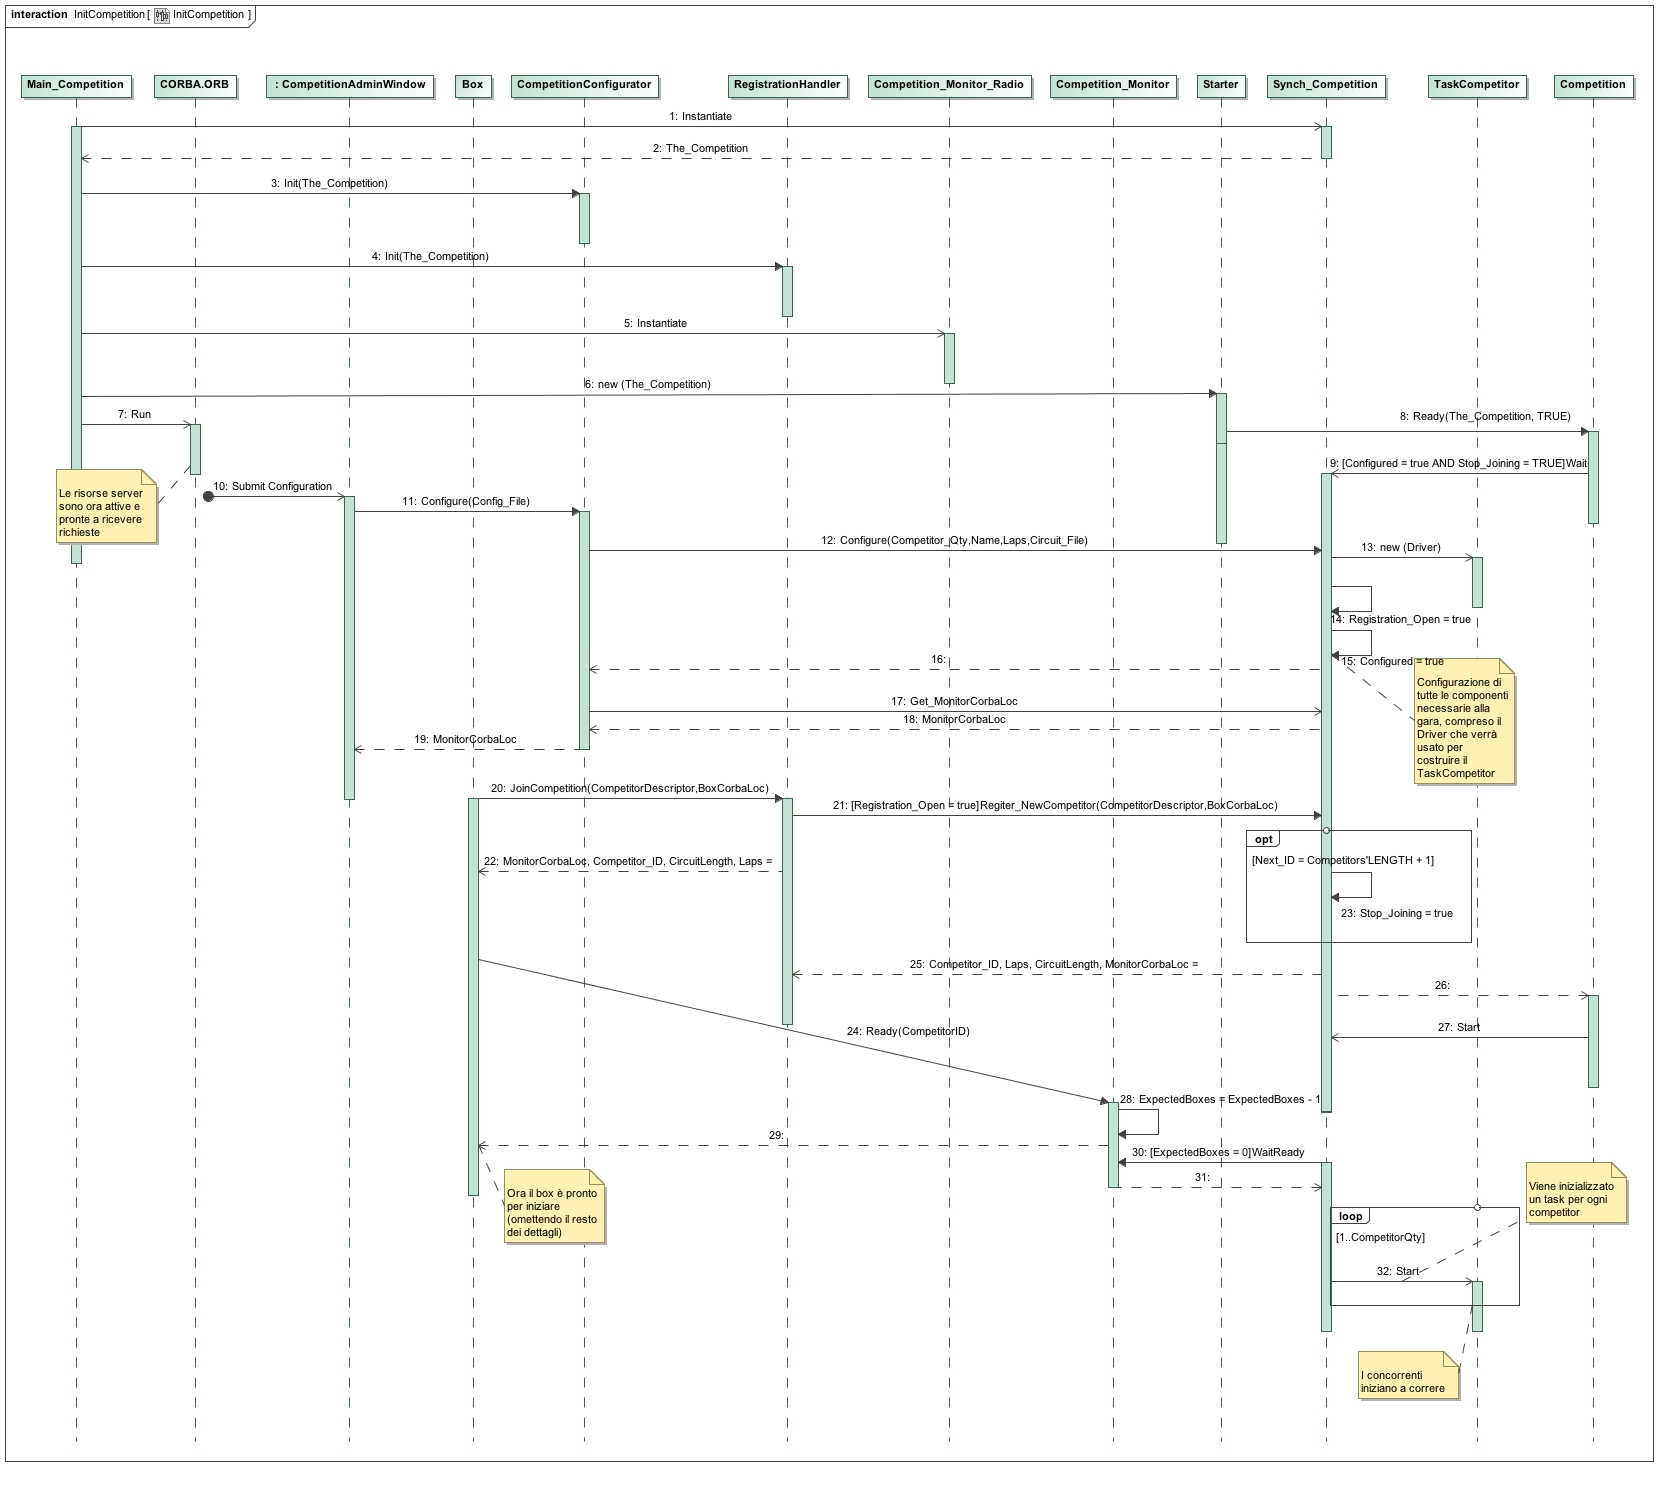
\includegraphics[angle=90,scale=0.35]{img/SequenceDiagrams/InitCompetition.jpg}
\caption{Sequence Diagram - Inizializzazione competizione}
\end{figure}
\end{center}
\clearpage
Una volta avviato il main della competizione, per prima cosa vengono
inizializzati tutti i server, vale a dire \textbf{CompetitionConfigurator},
\textbf{Registration\_Handler} e \textbf{Competition\_Monitor\_Radio}. Viene
avviato
un task \textbf{Starter} che rimane in attesa
della configurazione e registrazione concorrenti avvenuti per dare lo
\underline{Start} alla gara. Viene inoltre allocata una risorsa protetta di tipo
\textbf{Synch\_Competition} pensata
per agevolare la fase di init. Ne viene condivisa un'istanza fra
\textbf{CompetitionConfigurator}, \textbf{Registration\_Handler} e
\textbf{Starter}.
Tale risorsa permette di regolare i vari step dell'inizializzazione. Finch\`{e}
la competizione non viene configurata (dal passo \textbf{10} al passo
\textbf{16}),
non sar\`{a} concesso di registrare concorrenti. Una volta configurata la
competizione, viene aperta la guardia \textsc{Registration\_Open} e il metodo
\underline{Register\_NewCompetitor} potr\`{a} essere invocato (in
\textbf{Synch\_Competition}). L'iscrizione dei concorrenti avviene a partire dai
\emph{Box}.
Nel diagramma l'azione iniziale del \emph{Box} è la \textbf{20}. In realt\`{a},
nel nodo del box, viene prima avviato uno script che esegue il main del box
seguito dal main dell'interfaccia (java) di configurazione del concorrente e del
box. A configurazione avvenuta, i parametri vengono inviati al server della
competizione invocando il metodo del server \textbf{Registration\_Handler}
\underline{Join\_Competition}, come scritto nel diagramma. A iscrizione
avvenuta, 
i parametri di configurazione della competizione tornati vengono usati per
inizializzare e avviare il box e relativi task grazie a cui successivamente
sar\`{a} possibile mandare il messaggio di \underline{Ready} alla competizione.
Quando tutti i concorrenti sono stati registrati (\textbf{23}), bisogna rimanere
in attesa della conferma di avvenuta inizializzazione dei \emph{Box}. Ci\`{o}
avviene quando il thread del task \textbf{Starter} invoca il metodo
\underline{Start} del \textbf{Synch\_Competition}, dentro cui viene messo in
attesa
sul \textbf{Competition\_Monitor} tramite \underline{Wait\_Ready}. Quando tutti
i \emph{Box} hanno dato l'ok, significa che sono pronti per ricevere
richieste dai rispettivi competitor e la gara pu\`{o} cominciare. Vengono
cos\`{i} avviati uno ad uno (\textbf{32}) e la competizione ha inizio.
\subsection{Stop competizione}
Lo stop del sistema avviene su 3 livelli: stop dei task, stop delle interfacce
utente e stop dei server. Vediamo in dettaglio:
\begin{description}
\item{\textbf{Stop dei task}}:\\
i task che devono essere fermati sono i \textbf{Competitor\_Task} lato
competizione e i task \textbf{Update\_Retriever} e \textbf{Strategy\_Updater}
lato box.
I primi si fermano in automatico quando le condizioni dell'auto non permettono
di procedere (benzina finita o gomme troppo usurate) oppure a competizione
finita
(fine ultima lap). I secondi due si fermano quando l'aggiornamento fornito dal
monitor della competizione segnala uno stato dell'auto a causa di cui il 
concorrente non pu\`{o} procedere (poca benzina o molta usura gomme), oppure
quando il concorrente finisce l'ultima lap (sempre grazie agli aggiornamenti);
\item{\textbf{Stop delle interfacce utente}}:\\
\`{e} sufficiente chiudere le interfacce con il tasto \textbf{x} in alto a
destra;
\item{\textbf{Stop dei server}}:\\
una volta finita la gara e chiuse le interfacce utente, lo script di avvio
procede l'esecuzione invocando un \textbf{killall -9} sui main avviati,
interrompendo
cos\`{i} anche i task server.
\end{description}